\documentclass[a4paper]{article}
%\documentclass{scrartcl}
%\setkomafont{disposition}{\normalfont\bfseries}

% environment
\usepackage{fancyhdr} % this is needed to include headers
\usepackage{lastpage} % this is needed to include numbered pages
\pagestyle{fancy}
\usepackage{graphicx} % this is needed to include figures
%\usepackage{lipsum}
\usepackage{pdflscape}
\usepackage{hyperref}
\usepackage{verbatim}
\usepackage{amsmath}
\usepackage{algorithmic}

\fancypagestyle{rest}
{
\fancyfoot{}
\fancyhead[L]{The RuleR Tool}
\fancyhead[R]{\leftmark}
\fancyfoot[C]{Page \thepage\ of \pageref{LastPage}}
\fancyfoot[L]{COMP30040}
\fancyfoot[R]{2016/2017}
}
\fancypagestyle{firststyle}
{
   \fancyhf{}
   \fancyfoot[R]{\today}
   \fancyfoot[L]{The University Of Manchester}
}

%\usepackage{fancyhdr}
 
%\pagestyle{fancy}
%\fancyhf{}
%\rhead{Share\LaTeX}
%\lhead{Guides and tutorials}
%\cfoot{Page \thepage\ of \pageref{LastPage}}
%\usepackage[a4paper]{geometry}

%\usepackage[cm]{fullpage}
%\pagestyle{myheadings}
%\markright{Mantas Daraciunas\hfill Sequence diagram\hfill Software Engineering \hfill}
%\cfoot{\thepage\ of \pageref{LastPage}}
% change the margins of the page
%\usepackage[margin=0.6in]{geometry}
%	\addtolength{\textwidth}{1.75in}

\addtolength{\topmargin}{-.2in}
% now set up a simpler command to wrap the inclusion of SQL scripts
\newcommand{\includesqloutput}[1]{\tiny \lstinputlisting{#1} \normalsize}

%%%% Start a new document
\begin{document}

% make sure that you change the next line to the correct exercise number
\title{
\large COMP30040 Third Year Project
\\[0.7cm]
\textbf{\huge Runtime Verification Tool\\ using RuleR Language} 
}

% your full name goes here, and do not forget your student ID
\author{\Large Mantas Daraciunas} 
\date{}
% remember to copy this template and change the name of the file
% according to the rules in the Practical Sessions Manual

% now LaTeX prints the title, author name, etc. here
\maketitle
\thispagestyle{firststyle} % remove page numbering on first page
\newpage % start a new page

%%%
%  Create a new section and include the answer for each task as a subsection
%%%
\tableofcontents
\pagestyle{rest}
\newpage
\section{Requirements}

To create a tool which is able to monitor the events in runtime and decide whether the sequence of the events has happend according to the rules provided. 

\newpage
\section{Descriptions}
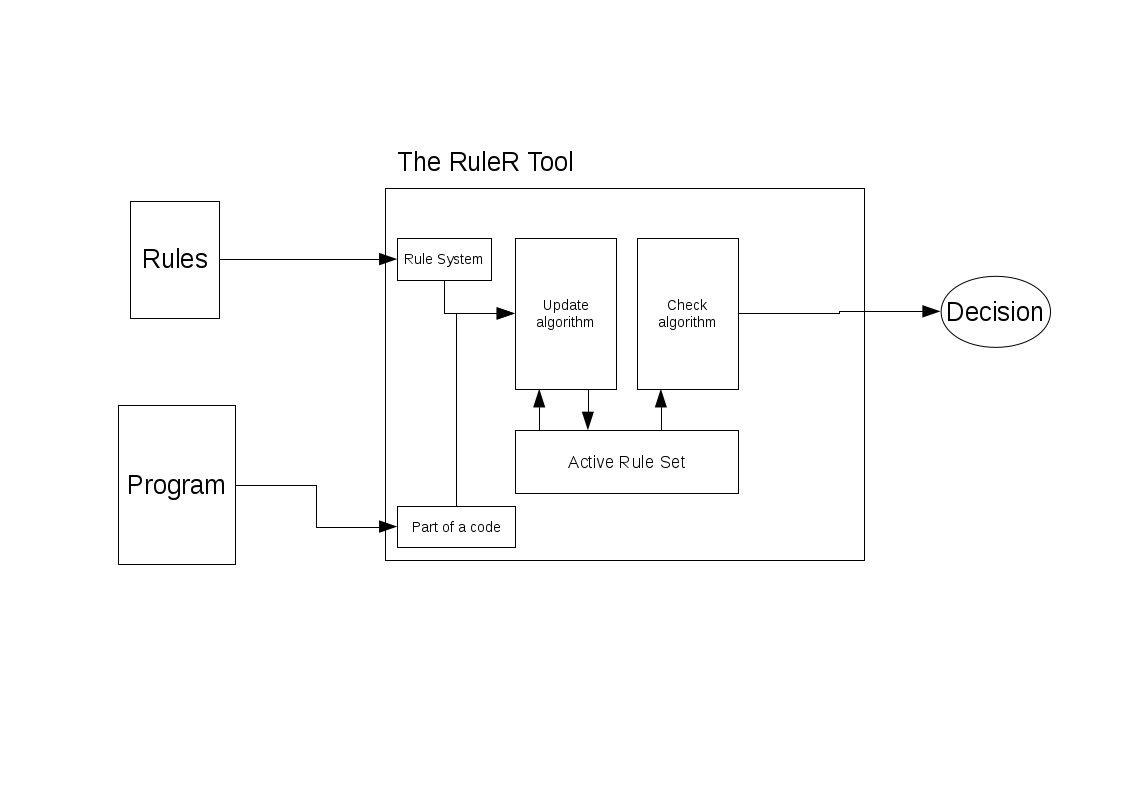
\includegraphics[width=\textwidth,height=\textheight,keepaspectratio]{../Graphs/overallProcess.png}

\vfill

\textbf{Rule System} – Predefined set of rules which define the expected flow of the program. Rule System should contain one or more rules. Each rule has to have list of the events with optional conditions which will lead each event to some action – another rule or verdict (success or failure). A Rule is of the form
\[
Modifier RuleName(Parameters) \{
List[RulePart]
\}
\]
where\\
Modifier = always or state or step\\
RulePart = EventName(Parameters) [Optional Conditions] -> List[Action]\\
Action = RuleName(Parameters) or Ok or Fail\\


The \textbf{Modifiers} of the rule can be as following:\\
always = always keep this rule activation\\
state = remove this rule activation if it ‘fires’\\
step = only keep this rule activation for one step\\

A \textbf{Rule System} is a tuple < R, S, F, A >\\
where R is a set of Rules,\\
S, F and A are sets of starting, forbidden and asserted rule names.\\
S must contain at least one rule name.\\
F and A may be empty 

\vfill

\begin{comment} 
\underline{Each Rule System will have main, very first rule which will hold the modifier always to it. This means that this rule will be checked in the end of Active Rule Set every time we investigate new event. This will be a start point for in a very beginning and crucial if none of the rules were matches during Update stage. 
You are correct to say that it is usual to have a single Start rule written first and for that rule to be an always rule… we almost never do anything else. But technically a rule system can be more flexible.}
\end{comment}

\vfill

\textbf{Active Rule Set} – is a set of the current activated rules in the monitored trace. Rule Activations are represented as rule name with the parameter and value. Each rule could have more than one Rule Activation in Active Rule Set 

\vfill

\textbf{Update stage} – the part of runtime verification tool which updates rules in Active Rule Set. It takes piece of code and rule from Rule System and replaces, deletes, introduce or keep existing rules in Active Rule Set.\\
The update algorithm takes an event and naively does the following\\

\begin{algorithmic}
\FOR {each rule activation <ruleName, binding> in the Active Rule Set}
  \FOR {foreach RuleBody in ruleName}
    \IF {the event matches the left of the RuleBody}
      \STATE write the binding 
      \STATE update the binding and use it to add the right side
      \IF {the modifier of RuleBody is state}
        \STATE remove the rule activation
      \ENDIF
      \IF {the modifier of step} 
        \STATE then remove the rule activation
      \ENDIF
    \ENDIF 
  \ENDFOR 
\ENDFOR 
\end{algorithmic}
\vfill
The stuff to do with bindings we should discuss at a later date, when you need to implement the update algorithm. \par

\vfill

\textbf{Decision stage} - the part of runtime verification tool which takes Results of each rule from Active Rule Set and generates a decision on to the screen.
The decision algorithm produces a verdict after each event. It uses the Active Rule Set and the sets A and F to do this.\\
Approximately it decides as follow, where ARS is the Active Rule Set:
\begin{algorithmic}
\IF {Fail is in ARS} 
  \STATE decide Failure
\ELSE
  \IF {the ARS is empty}
    \STATE decide Success
  \ENDIF
\ELSE
  \IF {we have not just fired a rule in A}
    \STATE decide Failure
  \ENDIF
\ELSE
  \IF {there is a rule name in ARS that is also in F}
    \STATE decide WeakFailure
  \ENDIF
\ELSE
  \STATE otherwise decide WeakSuccess
\ENDIF
\end{algorithmic}

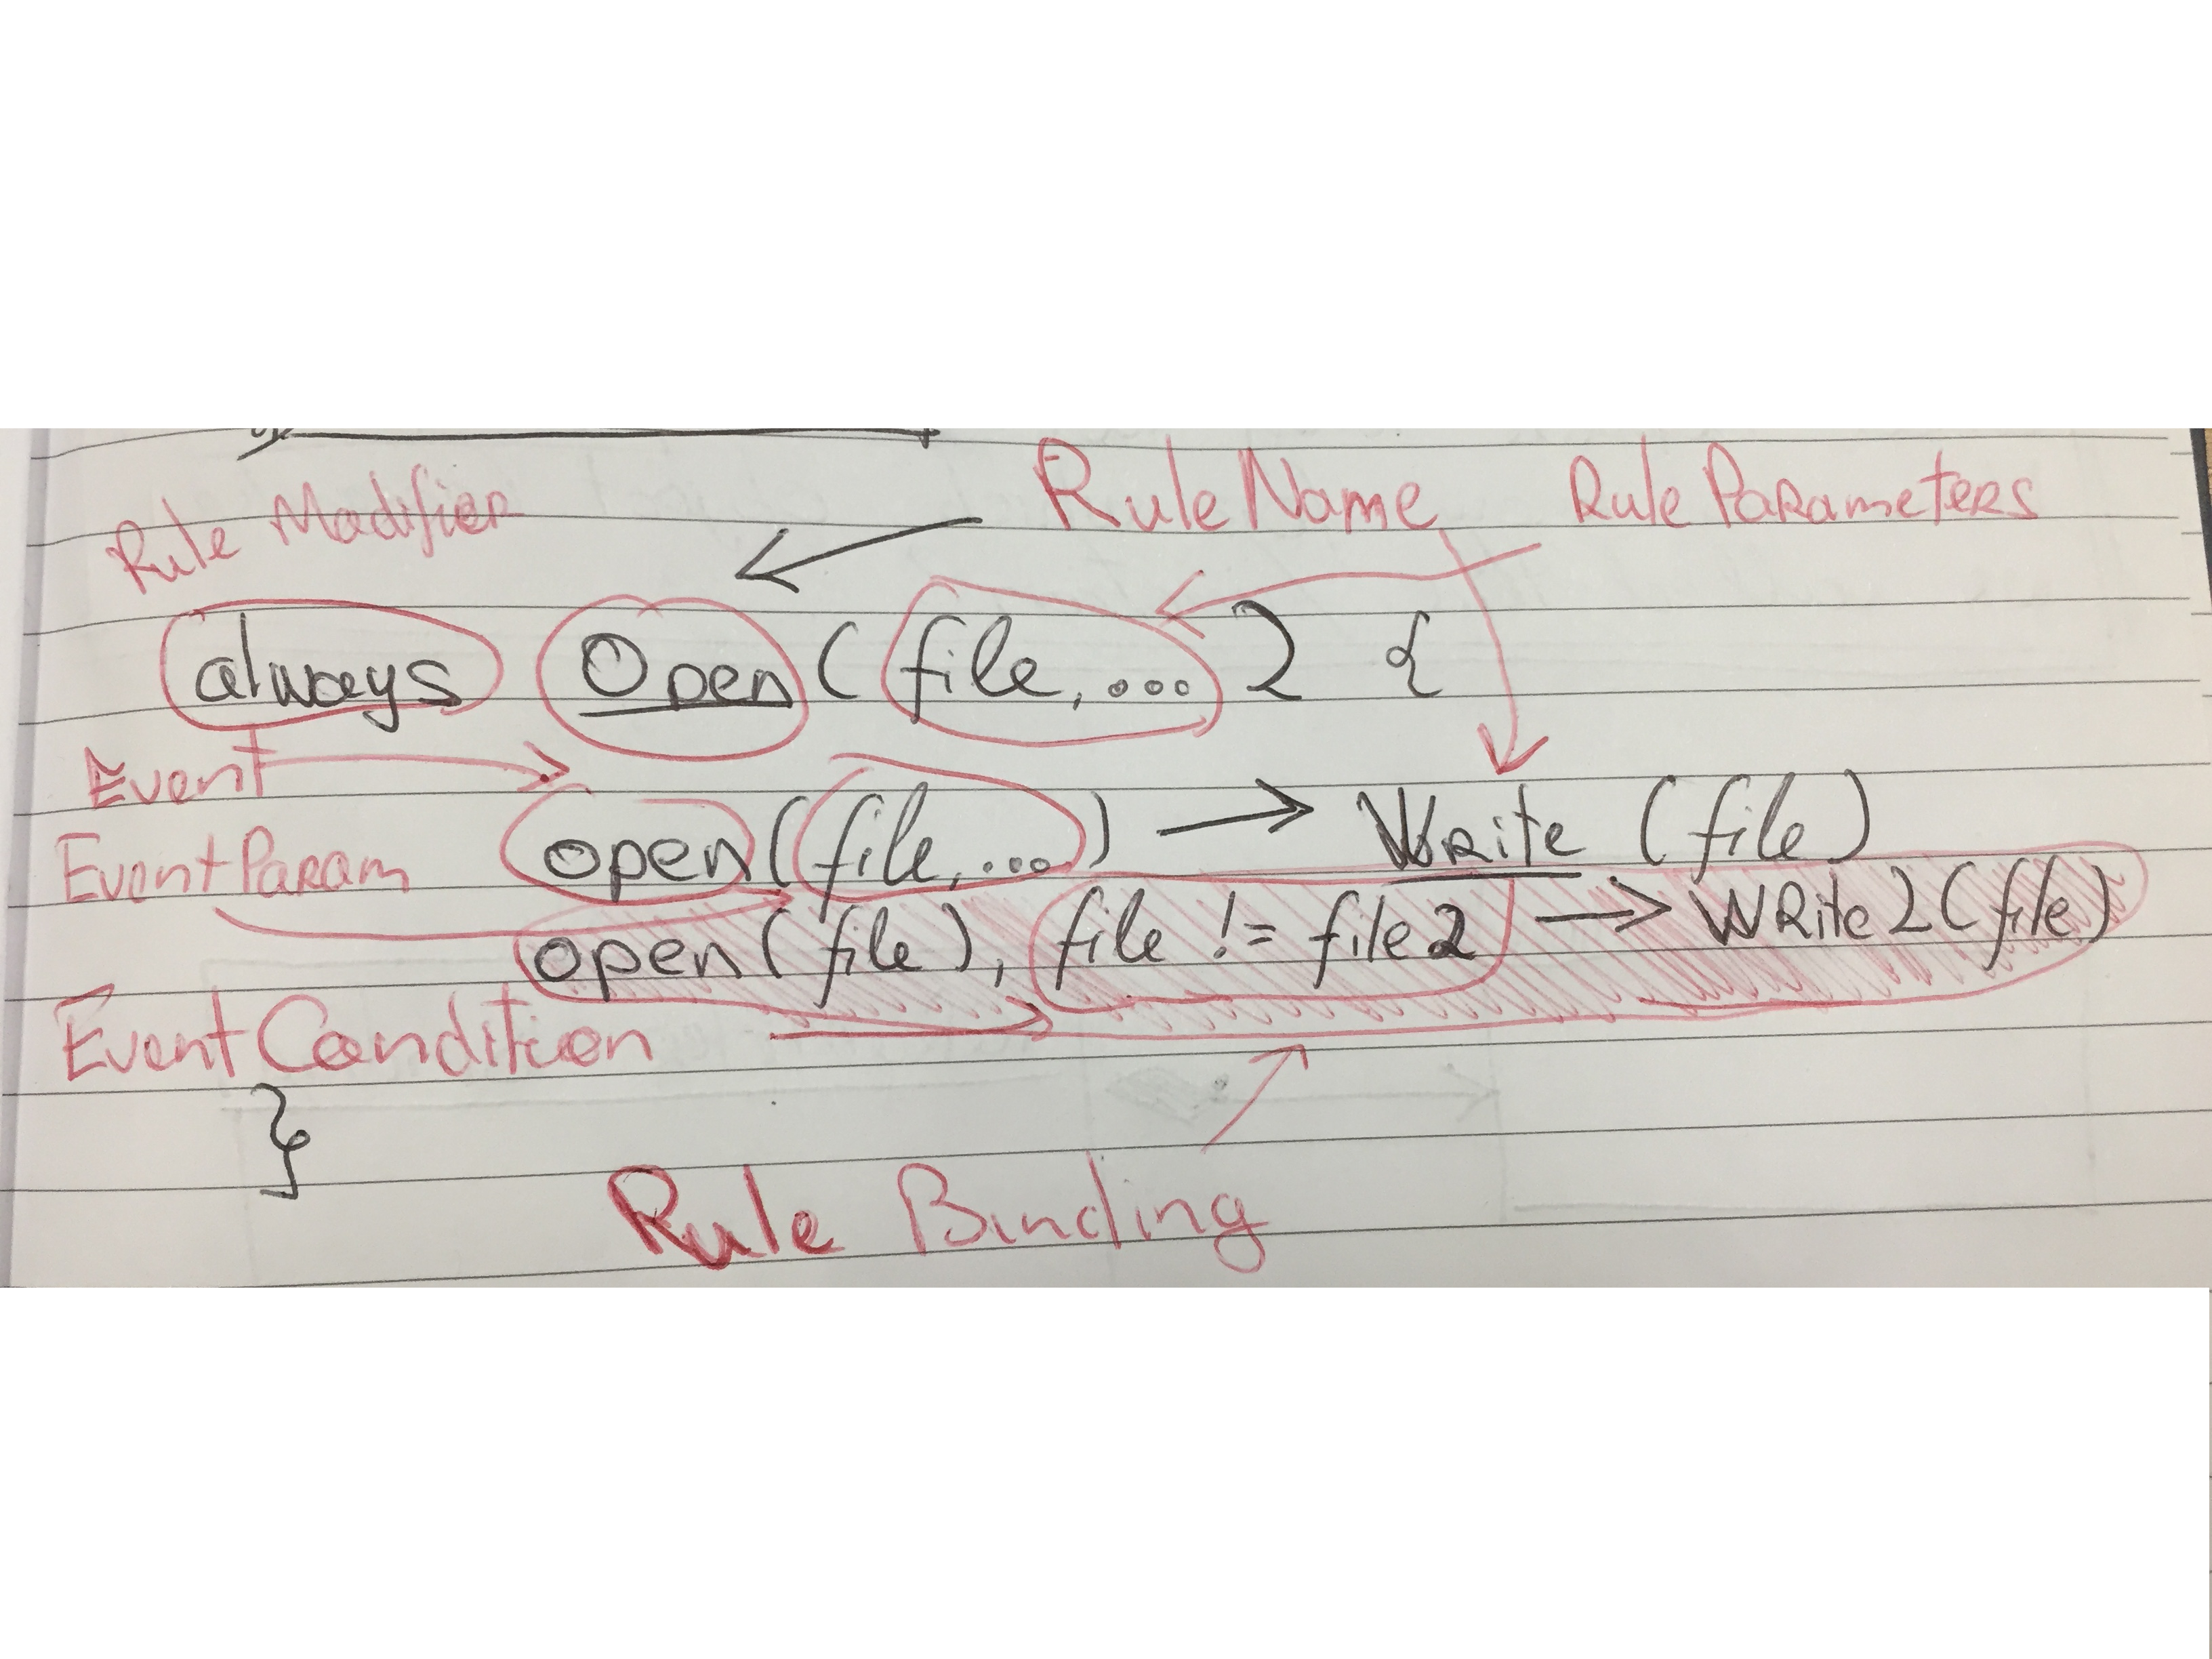
\includegraphics[width=\textwidth,height=\textheight,keepaspectratio]{../Pictures/image1.png}
\includegraphics[width=\textwidth,height=\textheight,keepaspectratio]{../Pictures/image2.png}

\newpage

\section{Design}
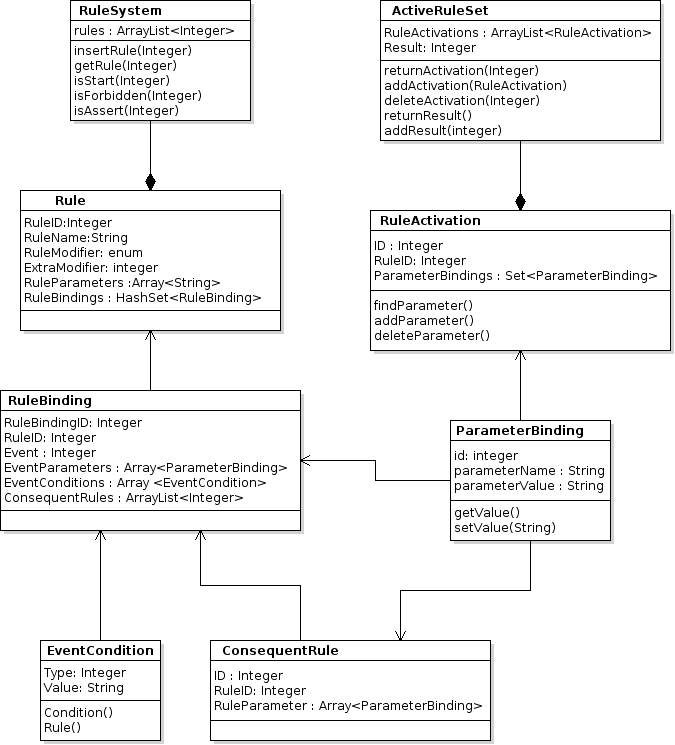
\includegraphics[width=\textwidth,height=\textheight,keepaspectratio]{../Graphs/classes.png}

\begin{comment}
\section{Rich Picture}
\includegraphics[width=\textwidth,height=\textheight,keepaspectratio]{../Downloads/Presentation1.png}
\newpage

%-----------------------------------------------------------------

%============= Work System Analysis =======================

%----------------------------------------------------------------

\section{Work System Analysis}
\subsection{Customer}

  \begin{enumerate}
    \item Customers of the business” Well Renowned Burger” can be local people as they are near the café and has a bigger chance to go into the café and buy a burger as a meal. 

    \item Customers can be people who likes burgers and would consume fast food. 

    \item People willing to waiting for a tasty burger, because when it is peak time, it take a long time to be served.

    \item People who have bank card, the café offer card payment.

    \item People who would like a table for a meal, as the café offer tables and seats.
  \end{enumerate}

\subsection{Future Customers}
  \begin{enumerate}
    \item People have mobile phone, tablet or a PC that has access to the Internet, as the café is proposing an online menu, online shopping basket, online table reservation system and delivery system.

    \item People using social media, as the café is proposing a delivery system using social media.
  \end{enumerate}
\subsection{Product / Service}
  \begin{enumerate}
\item The café offers food and drink, burgers, which is what the café mainly offer.

\item The café also offers table and seats for customers.

\item The café offers card payment to those customers who would like to pay by card.
  \end{enumerate}
\subsection{Future Service}
    \begin{enumerate}
\item The café will offer online menu and online order system, so that customers can order online and collect in store.

\item The café will offer online table reservation system for customers to reserve table online.

\item The café is proposing a “crowd source delivery” system to deliver food order to customers.

\item The café will offer loyalty points scheme, that customers get points for every purchase.
  \end{enumerate}
\subsection{Current Business Process and Activities}
  \begin{enumerate}
\item Receive order from customers and receive payment form customers.

\item Put order through the Kitchen.

\item Receive food from the kitchen and give them to the customers
  \end{enumerate}
\subsection{Future Business Process and Activities}
  \begin{enumerate}
\item Receive online table reservation information.

\item Inform customers when table is available.

\item Receive order from customers or online and receive payment or payment details form customers.

\item Put order through the Kitchen.

\item Receive food from the kitchen and give them to the customers or deliver to customers.

\item Add up loyalty points in customers' accounts.

\item Automatic notifies the food wholesaler as and when stocks need replenishing.
  \end{enumerate}
\subsection{Participants}
  
Employees :
\begin{enumerate}
\item Customers who make the order.

\item Assistants who take the order.

\item Staff in the kitchen.

\item Delivery service.
\end{enumerate}
Outside of the business:
\begin{enumerate}
\item Food wholesaler

\item Drink supplier
  \end{enumerate}
\subsection{Information needed for current business}
  \begin{enumerate}
\item Order information.

\item Payment Information.

\item Stock information.

\item Wholesaler information.

\item Tax rate.

\item Price of the stock form wholesaler.
  \end{enumerate}
\subsection{Future Information}
  \begin{enumerate}
\item Loyalty points account information.

\item Table reservation information.

\item Identification and address of customer.
  \end{enumerate}
\subsection{Currently used Technology}
  \begin{enumerate}
\item Payment method.

\item Till.
  \end{enumerate}
\subsection{Technology in the future}
  \begin{enumerate}
\item Internet

\item Online order system

\item Online shopping basket

\item Online table reservation system
  \end{enumerate}
\subsection{Strategies}
The strategies of the business now is to increase the competitive, reduce the loss of custom during peak hours and maximise potential customers. In order to do that, the business needs to minimise the waiting time and increase the efficiency of their work by introducing new online technology to satisfy customers' needs.
\subsection{Infrastructure}
  
The infrastructures required to running the current business are as below:
\begin{enumerate}
\item Food Wholesaler,

\item Drink Supplier,

\item Delivery service from supplier to the café,

\item  Energy and water,
\end{enumerate}
Infrastructure needed for future business:
\begin{enumerate}
\item Internet,

\item Online system programmer,

\item Delivery service form café to customers,
  \end{enumerate}
\subsection{Environment}
  \begin{enumerate}
\item UK laws and regulations,

\item Independent Business,

\item Competitive market,
  \end{enumerate}
\newpage

%-----------------------------------------------------------------

%============= Porter's Value Chain Model =======================

%----------------------------------------------------------------

\section{Porter's Value Chain Model}
\subsection{Support Activities}
\subsubsection{Firm Infrastructure}
  \begin{enumerate}
 \item Introduce new technology to reduce the waiting time of customer to be served in order to reduce customers lose and attract more customers

 \item Introduce new service (Delivery, table reservation and loyalty points) to reduce customers lose and target new customers
  \end{enumerate}
\subsubsection{Human Resource Management}
  \begin{enumerate}
   \item recruit a delivery driver for the delivery service

 \item recruit a team of IT programmer to program the online menu, online shopping basket, table reservation system, automatic stock ordering system, online loyalty points system and online customers' account database.
  \end{enumerate}
 
\subsubsection{Technology Development}
Introduce new mobile technology and new systems (online menu, online shopping basket, table reservation system, automatic stock ordering system, online loyalty points system and online customers' account database)
\subsubsection{Procurement}
Getting stock from organic fresh wholesaler
\subsection{Primary Activities}
\subsubsection{Inbound Logistics}
Organic fresh stock
 
\subsubsection{Operation}
  \begin{enumerate}
   \item Fast serve food

 \item Small Working place
  \end{enumerate}

\subsubsection{Out bound Logistics}
  \begin{enumerate}
   \item Unbelievably good taste in spite of the decor

 \item Delivery to door

 \item Take short time to get food after ordered
  \end{enumerate}
 
\subsubsection{Marketing \& Sales}
  \begin{enumerate}
   \item Stable price  

 \item target at people who like a convenience meal

 \item Online menu and order
  \end{enumerate}
 
\subsubsection{Service}
  \begin{enumerate}
   \item Table and Seating in café 

 \item Delivery service

 \item Loyalty points scheme
  \end{enumerate}
\newpage

%-----------------------------------------------------------------

%============= PESTLE Analysis =======================

%----------------------------------------------------------------

\section{PESTLE Analysis}

\subsection{Political}
The standard tax rate in UK is 20\%, restaurants are required to pay taxes annually. The rate is for drinks and food to be consumed on the premises. Food politics has created a cultural backlash that is against mechanised food. The Northern Quarter specialises in local food, which is a collaborate effort to build self-reliant food economies in a particular area. It reduces the long distance shipping by larger corporate companies and uses local farmers and producers of food.
The use of organic products in ‘Well Renowned Burger’ helps to promote animal welfare.  This is the general health and well being of animals from exploitation to abuse. For organic products, the welfare requirements are higher, such as the health and food for the animal is a higher quality. Organic farming means that the animals need few if any antibiotics, with it only being used to treat sick animals. Intensive farming uses it to prop up a fundamentally unhealthy routine, which weakens the immune system. Many consumers look for organic foods as they have higher welfare food choices.
\subsection{Economic}
The United Kingdom has one of the largest national economies in the world, and the service sector dominates the UK economy, which contributes around 78\% of GDP. For 2014, the annual GDP growth rate is about 3.2\%, which is 11 years high since 2003, this shows the UK economies is growing strong since the economic crisis in 2009, which means people are more willing to spend on food/luxuries. However, it may increase the inflation rate in UK, this will affect the price for ‘Well Renowned Burger’, therefore money would get less valuable, and price increasing may affect the sales, and ultimately it will affect the profit. Since the economy in UK is growing stronger, the unemployment rate is falling as well.  According to the latest Office for national Statistics (ONS) figures, Unemployment fell by 600,000 to 1.96million from Jan 2013 to the end of September 2014. As more firms are likely to employ more people, if  ‘Well renowned burger’ would have to employ more workers, it requires more wages. Therefore, less profit from the business.
\subsection{Social}
 A lot of people usually find the Northern Quarter area through the popular Arndale Shopping Centre, which is situated nearby. So many consumers are shoppers who are looking for a place to eat without having to travel so far or they would like to try something new that is not already in the city centre. The existing shops open are cafes/local shops and bars mainly, so it is a popular area to meet others and enjoy company.  The main population of Manchester is between the age of 25-44 (33.4\%) and 16-24 (19.5\%) sourced from the Manchester City Council. Many of these ages would be the main demographics that are likely to go to Northern Quarter shops for meeting/to eat/ shop or for the various clubs at the area. ‘Well Renowned Burger’ will have to create a appropriate branding which either caters towards a main audience or it is suitable for all different ages. The most suitable age range would be aged 16-44 as it is the main population of Manchester; hence it will have more consumers. It is also appropriate to have décor that will attract consumers into the restaurant.
\subsection{Technological}
 Technology can be an efficient tool to aid businesses or to make a task much easier. Most of the cafes set up its own order management system to improve the efficiency and reduce the time from ordering and processing. It also helps to record the order details, which can avoid problems from recording with paper such as record being unorganised; workers may find it difficult to track orders.  Also it can provide detailed information about the sales of certain food. Besides that, cafes often provides Wi-Fi connections for customers, as it keep customers to stay in for longer and it helps to increase the customer loyalty as customers may visit again for the Internet connection. Other than that, restaurant often advertise through online social web site such as Facebook/twitter, it helps the restaurant to provide more information about themselves, such as promotions.
\subsection{Legal}
 There are some regulation and legislation that restaurants have to follow. An example would be the ‘Food Hygiene Rating Scheme’ (FHRS) in the United Kingdom, which gives consumer information about the hygiene standards in restaurants, takeaways or food shops based on the rating from 1-5 (Highest to lowest). These ratings help consumers to understand the hygiene level before visiting the restaurant. For “Well Renowned Burgers”, the décor is described as ‘grubby shelves, cardboard boxes and graffiti-strewn walls’, which can potentially put off consumers. A high rating advertised could eliminate their worries.
Besides that, labour law is important to be mentioned, as every food shop will be required to employ a number of workers to run the business. The UK labour law helps to protect workers benefit from a minimum charter of employment rights. An example would be the National Minimum Wage Act; workers who are over 21 years old have the right to a minimum wage of £6.50. This is important for shop owners as it will contribute to the fixed costs for the business.
\subsection{Environmental}
The location is situated in the northern quarter of Manchester. In 2014, it is the second worst area in Manchester for crime rate, with the most violent being Gay Village. Since there are lots of bars, so there would be a lot of after-hours drinkers, which can make the area dangerous during the late night.  
The economic impact of tourism in Manchester was estimated at £6.6 billion in 2012 according to Visit Manchester, with many tourists located around the city centre. So there are many potential consumers that can visit the location of the restaurant easily. The environment of the Northern Quarter is famous for being a centre for alternative culture and a hub for numerous bars and cafes/restaurants, so the ‘Well Renowned Burger’ will have a lot of competition in the area. Over time, certain types of business were attracted to the area, which offered low rents. This became the main strength of the Northern Quarter —it is now known for the independent stores, cafes and bars, and for offering a distinct alternative to the shopping experiences to be found elsewhere.
\newpage

%-----------------------------------------------------------------

%============= Porter's Competitive Forces and Strategies =========

%----------------------------------------------------------------

\section{Porter's Competitive Forces and Strategies}
\subsection{Threat of rivalry}
Customers may go to other restaurants with better décor as ‘Well Renowned Burger' has ‘beaten up wooden tables and chairs, grubby shelves, cardboard boxes and graffiti – strewn walls. There are no prices given for the café so it cannot be compared to others, the description of the burgers are ‘unbelievably good' but with only 2 options that it specialises in, many people may consider going to other restaurants as there is a limited option.
With only 20 seats, many customers would not like to wait with 2 other employed workers, the food production will be slow, and the customers may be in a rush and will look for other substitutes. The competitors are all the cafes in Northern Quarter. However, the main competitor will be ‘SoLiTa' and ‘Almost Famous' which are both popular burger restaurants in Northern Quarter. Both seats more than 20 and both hire a lot of stuff. Some people may prefer to seat in a smaller place, as it is more peaceful.
The décor in both are American diner styled which is more themed than the ‘Well Renowned Burger', so there is a high chance that customer may prefer to dine in a more comfortable area with similar food being offered.
The organic food can be defined as having food quality, human health, environmental, animal welfare and socio-economic aims - which derive more from a consumer perspective than from a producer perspective. The result is that ‘Well Renowned Burger' has a very strong brand image in the eyes of consumers; this can set it apart from other competitors.
Many of the competitors have a website which shows the menu online and also a phone number to make bookings. The suggestion of making orders to pick up for ‘Well Renowned Burgers' with a registered profile seems like a inefficient way. The consumers would not like to register a profile on the website to order a burger. For an order, most people would rather order through a phone so that it is easier and they can be alerted.
 
\subsection{Threat of Substitutes}
Production costs are minimal as they only make burgers, so there is not much ingredients to buy. Since the produce is organic, it may be more expensive in price but is usually sourced locally. In terms of branding, the café specialises in burgers. There are many cafes or restaurants that specialise in the same type of food such as ‘Almost Famous' and ‘SoLiTa', which both have a loyal customer fan base. Therefore the product sold is not different or new in the northern quarter. However, even the décor is poor with bad service, the restaurant still managed to attract a large number of customers to queue up for its fresh organic burger.
The suggestion of a table reservation system is effective; the booking system should include details such as party size, name, and details, which they can be easily contacted by. This maximises the potential of her business and increases the customer loyalty, as they would not have to queue instead.
In the industry, American burger joints overall, sales exceeded \$72 billion, and while that was up 1.2\% from the previous year, if not for higher prices the number in fact would have declined. However, it's also a reflection of other causes, such as health considerations, as there are now about 1 million restaurants nationwide, along with the option to simply eat at home — and dietary changes. Smaller chains of burger stores (Five Guys and Smashburger)  have reported a higher percentage rate of sales than the fast food joint such as Burger King or McDonald's, with a sales growth of 10.4\%. This shows that consumers are beginning to spend their money on more quality burgers rather than the cheap value which is given by fast food stores. The ‘Well Renowned Burger' can benefit from these statistics if the burgers are true to tasting 
'unbelievably good'.
 
\subsection{Barriers to entry}
The ‘New York' styled burger is simple to be produced and organic ingredients can be easily purchased from the market at a higher price than conventional food items. Since Northern Quarter has many restaurants and cafes that provide similar burgers, a new restaurant may introduce an organic burger as their unique selling point with better décor and more staff to provide better service. Besides that, Northern Quarter is right in the Manchester city centre, a very popular place for gathering; since a profitable market always invites more competition. Also the restaurant has so many problems that can be countered, newly joined competitors would definitely take an advantage of it. Other than that, Fast food industry has no legal barrier, so overall the threat of new entrants is high for ‘Well Renowned Burger'.
 
\subsection{Buyer power}
Buyers have a high bargaining power; even though customers visit the restaurant would only purchase a low quantity of burgers. The restaurant will be a local one so it will rely heavily on the consumer. The décor in the restaurant is badly designed and also the service is low so the buyer may go for other restaurants. The owner will have to think about changing these factors so she is able to keep the consumers coming to the restaurant to keep the business running.
The use of social media is important to spread the word of the restaurant and potentially increase profits. The idea of ‘crowd source delivery' using social media is not effective though. It can prove to be unreliable as customers delivering on behalf of the café is not very safe to be delivered from strangers.
Another suggestion is to have a loyalty point scheme for every purchase in ‘Well Renowned Burger'. It is a good idea to increase loyalty for the buyers but it lowers the profit slightly. The point scheme also motivates the customer to keep coming back to the restaurant, which gives the power to the company more so than the buyer.
The brand identity of the restaurant is not very unique in Manchester as there are already many restaurants that provide this a style of food. The specials of ‘New York' burger are not unique and have already been done before in other restaurants, the company will have to create a special branding which makes it identifiable to consumers. The ‘Well Renowned Burger's main selling point that makes it unique from competitors is that it uses organic ingredients. This is different from many existing burger stores in the Northern Quarter. This also attracts a certain type of customer – the health and environment social type. The branding could be focused on this aspect of the food.
 
\subsection{Power of Suppliers}
There is a low threat of forward integration from the supplier, as they will only supply the organic meat and various toppings with the burger. The buyers will not usually look for organic burgers through the supplier, unless they visit the butchers or supermarkets regularly to make their own meals.
The importance of volume to the supplier will be that the ‘Well Renowned Burger' will have a low volume buyer, as it does not require a high amount of produce. The produce will not be fresh for a long time and the amount of seating means a limit of food being made daily. So the business is a low volume buyer, which means ‘Well Renowned Burger' will not have more marketing power from the supplier.
The mobile technology of having an automated stock system can be helpful in a retail setting, that can cause you to miss out on possible sales while you scramble to replenish your supplies, and also potentially hurt future sales figures if customers grow upset or dissatisfied with inadequate inventory. This however, will come at a cost which can hurt the potential profit made. It should only be used on a large scale company which has many different foods and not enough time to check all the produce.

\newpage

%-----------------------------------------------------------------

%============= BPMN for current system =======================

%----------------------------------------------------------------

\section{BPMN for current system}
\subsection{Current}
\includegraphics[width=\textwidth,height=\textheight,keepaspectratio]{./Downloads/original.png}
\newpage

%-----------------------------------------------------------------

%============= BPMN for new systems =======================

%----------------------------------------------------------------

\section{BPMN for new systems}

\subsection{Mobile Food Ordering System}
\includegraphics[width=\textwidth,height=\textheight,keepaspectratio]{./Downloads/mobile.png}
\subsection{Table Reservation System}
\includegraphics[width=\textwidth,height=\textheight,keepaspectratio]{./Downloads/table.png}
\subsection{Automatic Stock Ordering System}
\includegraphics[width=\textwidth,height=\textheight,keepaspectratio]{./Downloads/stocks.png}
\subsection{Crowd Source delivery}
\includegraphics[width=\textwidth,height=\textheight,keepaspectratio]{./Downloads/crowed.png}
\subsection{Loyalty point system}
\includegraphics[width=\textwidth,height=\textheight,keepaspectratio]{./Downloads/loyalty.png}
\newpage

%-----------------------------------------------------------------

%============= McFarlan's Strategic Grid =======================

%----------------------------------------------------------------

\section{McFarlan's Strategic Grid}
McFarlan's Strategic Grid shows the importance of Information Systems “Well Renowned Burger” currently use and will use in the future.
\\[0.3cm]
First of all, current information systems should be in “Factory” section, which means that currently used systems is quite important for business, however it does not look like it will be crucial for business in the future.
\\[0.3cm]
New Mobile Food Ordering System looks extremely important for café to reduce queues during peak times and maximise the potential of business. That is why, mobile food ordering system belongs to “Turnaround” section, which means that  it has big impact on future business strategy.
\\[0.3cm]
Customers who want to acquire table at the “Well Renowned Burger” café have to wait long time to get table. However, new mobile Table reservation system which allow people to subscribe their favourite table and get notification when it is free, will play crucial part for business. The place of this new system same as Mobile Food Ordering System is in “Turnaround” section.
\\[0.3cm]
Next on the list is Automatic Stock ordering system. This system might really help managers to deal with stocks, but it does not have huge impact for business itself. It will not help to reduce queues or serve people faster, thus the best for Stock ordering system is “Support” section.
\\[0.3cm]
“Crowed source delivery” system is very interesting and important for company. By people ordering online and other people delivering food to them “Well Renowned Burger” café will have shorter queues during peak hours and in that way they will maximise their profit. Therefore, “Turnaround” sections in McFarlan's Strategic Grid is the best place for this system.
\\[0.3cm]
Last but not least, Loyalty point scheme might attract new customers to café, however this system is not crucial for business to exist. Thus Loyalty point scheme should go to “Support” section.

\includegraphics[width=\textwidth,height=\textheight,keepaspectratio]{./Downloads/grind.png}
\newpage

%-----------------------------------------------------------------

%============= Conclusion =======================

%----------------------------------------------------------------

\section{Conclusion}

After using the seven models to analyze and understand Claire Voyant’s business ‘Well Renowned Burger’, there are several changes can be made to improve the business.
The décor of ‘beaten up wooden tables and chairs, grubby shelves, cardboard boxes and graffiti – strewn walls’ are not appealing to consumers and would not attract new potential customers into the restaurant. The importance of decoration creates a good atmosphere, which convinces the customer to stay longer or keep coming back. People are attracted to a restaurant more than just the good food, it is equally important to address the way that people feel inside the room too.
The branding of the restaurant does not seem to have a unique theme besides the organic aspect of the food. This branding could be used effectively to attract certain types of customer such as the environmental and health conscious. This could also potentially attract other customers who are choosing which burger restaurant to go to as the organic aspect makes the place seem more health friendly and they are less conscious of the animal welfare.
The specials ‘New York’ burgers have already been done in the competing burger stores in the Northern Quarter already. The type of food (burgers), which they specialize in, has increased in sales in the industry, with smaller chains making the best percentage of profit. This shows that the idea of food Voyant is going in is not decreasing in the industry.
The location of the restaurant, although competitive, is highly profitable as it is located in the City Centre. It is also close to the Arndale Shopping Centre so there is many shoppers which can o to the Northern Quarter to eat or relax. Although the area is not very safe at night, it will not matter to the restaurant, as it will not be open as late.
The restaurant does not cater towards a target audience; this can be negative especially in an area, which has a certain demographic of alternative people. Statistics from Visit Manchester show that the main age range is 25-44 in Manchester. So it is not recommended to create a burger restaurant aimed at a specific age range such as children. The best idea is to create a branding which is suitable for the ages specified.
The demographic of the Northern Quarter will for a local restaurant, which fits with the rest of the restaurants in the area. The use of local food in ‘Well Renowned Burger’ can help to reduce carbon footprint and it can help the economy of Manchester.
For the technological side of the restaurant, it is ideal to have the correct equipment for making burgers. An order management system would help to make tasks easier and provide information about sales. There should extra equipment, which can enhance the customers experience too, such as Wi-Fi or music for ambience.
\\[0.3cm] 
For the use of mobile technology suggestions, the online menu suggestion is a great way to interest people in visiting the restaurant; this can make a potential profit as they can see what is on the menu at the convenience of their mobile phones/computers. The idea to create a profile to be able to pick up orders seems inefficient though. Usually in a restaurant/café, customers would prefer to call with a mobile phone to order. An online ordering system would be ideal for a restaurant/takeaway with a wide range of food, but it seems unnecessary to create one with only burgers. This would be a waste of time to create a profile for the customer and a waste of money to develop this system.
The table reservation system is a great idea to make sure that customers get their seats in an efficient way. Some people may not like having to register a profile in order to do so on the website as they would rather just phone in an get it done instantly. So there should be an option to do that as well if people do not feel comfortable with the idea.
The idea of the ‘crowd source delivery’ is not a reliable idea. Although it can prove to be efficient and eco friendly, it is not safe to trust food to be delivered from people who are not hired into the business. The delivery could go wrong and the fault lies with the company.
The mobile technology of an automated stock system seems efficient to all restaurants, but in a small scale such as ‘Well Renowned Burger’, it does not seem necessary. It would cost for the system, which will lower the overall profit. With such as basic menu consisting mainly of meat, buns, toppings and side dishes etc., it seems not needed to use this system as there is not much on the menu so stock an be checked quickly by the manager. Also with the seating of 20, there will not be many a significant amount of stock sold within a day so the ingredients will not run out as fast.
The loyalty point scheme is also another good idea to increase the customer loyalty and their willingness to come back. It motivates the customer to spend more, however, it can decrease the profit made, as the points will go towards some sort of prize or freebie.

\newpage
\section{Slides}
\href{http://prezi.com/jwf9vcjoqqqn/?utm_campaign=share&utm_medium=copy&rc=ex0share}{Presentation at Prezi.com \\ http://prezi.com/jwf9vcjoqqqn/?utm\_campaign=share\&utm\_medium=copy\&rc=ex0share}

\end{comment}

\end{document}
